% ! TeX root = thesis.tex
\chapter{Introduzione}
Negli ultimi decenni, con la rapida crescita di dati e informazioni facilmente accessibili sul \textit{web}, è diventato sempre più semplice poter utilizzare, in parte o in tutto, le risorse reperite.
%
Tuttavia, l'uso improprio di tali risorse, senza attribuire i necessari crediti agli autori, costituisce, oltre che una pratica scorretta che contravviene a qualsiasi ordine deontologico, un illecito \cite{copyright-law-italia}.

In generale, l'atto di appropriarsi degli scritti di altre persone, in violazione della legge sul \textit{copyright}, viene definito \textbf{plagio} \cite{britannica}.

Anche nel mondo dell'informatica il problema del plagio è un fenomeno in crescita, incoraggiato per lo più dalla sempre maggiore quantità di progetti \textit{software} \textit{open source}, che induce gli sviluppatori a copia incollare frammenti di codice, talvolta neppure conoscendo le relative condizioni e termini di licenza.
%
Questo porta spesso a un uso improprio del codice altrui arrecando sanzioni e danni per lo sviluppatore.

Già a partire dagli anni settanta del novecento, sono stati proposti algoritmi e tecniche per l'analisi del codice, nonché l'identificazione e localizzazione di plagi.

In questo contesto è da porre in evidenza la differenza tra l'individuazione di cloni e quella di plagi.
%
Quando ci si riferisce a un clone, infatti, lo si fa con riferimento a un frammento di codice che è stata copiato e marginalmente modificato. 
%
Quando invece ci si riferisce ad un plagio si intende una sezione che è stata copiata e la cui opera di copiatura si è cercato di dissimulare, mediante opportune azioni di rifattorizzazione del codice \cite{muddu-et-al-2013}.  
%
Dunque, l'ambito di applicazione delle due ricerche è nettamente diverso: se nel primo l'obiettivo è quello di evidenziare il codice duplicato al fine di migliorare la qualità del codice e migliorare la manutenibilità del sistema, nel secondo lo scopo primario è identificare possibili condotte illecite.

Sicuramente, questo aspetto è, insieme alle prestazioni, la sfida principale da affrontare durante la progettazione di un sistema antiplagio.

\section{Problemi aperti}

\subsection{La rifattorizzazione del codice}
Come già anticipato, la capacità di un software antiplagio nel riuscire ad identificare possibili parti di codice plagiate, passa anche e soprattutto dalla capacità dello sviluppatore di saper rifattorizzare il codice.

In generale, non è possibile classificare tutti i possibili metodi con cui un programma può essere trasformato in un altro mantenendo inalterate le sue funzionalità.
%
Tuttavia, è possibile distinguere due macro categorie di modifiche: \textbf{lessicali} e \textbf{strutturali} \cite{joy-99}.

Le modifiche lessicali sono quelle che, in linea di principio, possono essere eseguite da un \textit{text editor} e non richiedono la conoscenza del linguaggio di programmazione con cui è stato sviluppato il codice. 
%
Alcuni casi esemplificativi sono:
\begin{itemize}
    \item la riformulazione di commenti, la loro aggiunta o rimozione;
    \item la riformattazione del testo, come l'introduzione di spazi vuoti, di nuove linee o il cambio dell'ordine dei parametri nella definizione delle funzioni;
    \item cambiare il nome degli identificatori e delle funzioni o i tipi di dato: ad esempio da \texttt{int} a \texttt{Integer} o da \texttt{float} a \texttt{double}.
\end{itemize}

Le modifiche strutturali sono invece fortemente dipendenti dal linguaggio di programmazione e richiedono un maggior sforzo in termini di comprensione della logica del codice.
%
Di seguito alcuni esempi di rifattorizzazioni che rientrano in questa classe:
\begin{itemize}
    \item aggiungere istruzioni ridondanti, come dichiarazioni, inizializzazioni, istruzioni di stampa;
    \item sostituire i costrutti di loop con costrutti equivalenti: passare, ad esempio, da \texttt{for} a \texttt{do/while};
    \item sostituire istruzioni \texttt{if} nidificate con dichiarazioni equivalenti, ad esempio \texttt{when} (in Kotlin) o \texttt{switch-case}, e viceversa;
    \item cambiare l'ordine di istruzioni indipendenti;
    \item cambiare l'ordine degli operandi: ad esempio \texttt{x < y} può essere cambiato in \texttt{y >= x};
    \item sostituire la chiamata a funzione con il corpo della stessa.
\end{itemize}

\begin{figure}
    \centering
    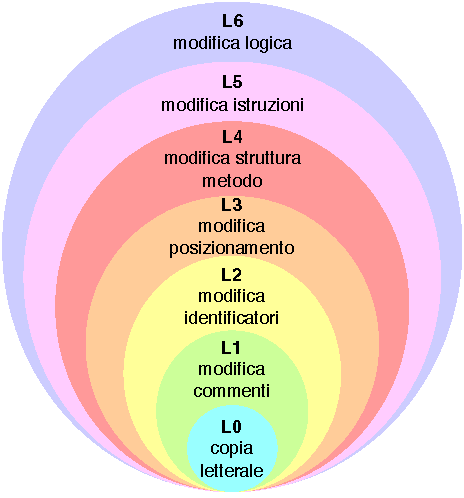
\includegraphics[width=0.5\textwidth]{resources/img/01-levels-of-plagiarism.pdf}
    \caption{Tassonomia dei livelli di plagio di Faidhi \& Robinson (1987).}
    \label{img:01-levels-of-plagiarism}
\end{figure}

Gli strumenti d'identificazione di plagi devono pertanto cercare di annullare, durante il processo di analisi, gli effetti di queste rifattorizzazioni.
%
A questo scopo le tecniche di analisi, introdotte nel \Cref{chapter:stateOfArt}, si compongono di più fasi nelle quali trasformano i sorgenti in rappresentazioni intermedie che astraggano il più possibile dai dettagli implementativi che possono essere facilmente cambiati, quindi applicano su di esse tecniche di \textit{matching}.

\subsection{Le prestazioni}
L'altro problema emergente nello sviluppo di un programma antiplagio che non si limiti a confrontare la similarità tra una coppia di progetti, bensì effettui un controllo uno a molti, in cui si testano tutte le possibili coppie, sono le prestazioni. 
%
Infatti, la maggioranza delle tecniche e degli algoritmi per effettuare i confronti sono inefficienti in termini di tempo costo. 
%
Questo è in larga parte dovuto al fatto che la misurazione della somiglianza tra una coppia di sorgenti ha una complessità almeno quadratica nel numero delle istanze delle sue rappresentazioni, e che, per ogni valutazione, il numero di confronti da effettuare è tipicamente elevato.

Questo problema è acuito dal fatto che i progetti \textit{software} stanno diventando sempre più complessi e si hanno a disposizione una quantità molto più elevata di dati e informazioni di quanto in passato si potesse immaginare.

Per questa ragione vengono sfruttate tecniche di parallelizzazione e devono essere adottate strategie di ottimizzazione in grado di ridurre il numero di confronti da effettuare e, quindi, diminuire il tempo di calcolo.
